\chapter{Methodik}
\todo{Eventuell Kapitel anders anordnen, sodass es einen besseren Lesefluss gibt.}
\label{chap:methodik}
Die Methodik dieser Arbeit beschreibt die wissenschaftlichen Hintergründe für das Vorgehen der Implementierung des Dashboards in einer \gls{dfir}-Umgebung für \oran. Der Fokus liegt auf der Integration von \gls{acema} und der (Weiter-)Entwicklung passender Visualisierungstechniken. Im Methodikteil werden die wissenschaftlichen Hintergründe über getroffene Entscheidungen erläutert. Zudem werden die Herausforderungen und Einschränkungen bei der Anwendung der Methoden reflektiert, um die Validität der Forschung kritisch zu beleuchten.
\section{Auswahl der empirischen Methode}
\todo{Kapitel umbenennen: Überschrift passt nicht. Du beschreibst, was die Methode macht, nicht warum du sie auswählst.}
\label{sec:auswahlDerEmpirischenMethode}
\gls{acema} ist \glqq eine umfassende empirische Methode zur Analyse von Bedrohungen in \oran Umgebungen \grqq (eigene Übersetzung: \autocite{klementSecuring6GTransition2024}). Die Integration der Analyse-Methode von \citeauthor{klementSecuring6GTransition2024} in das Forschungsprojekt \gls{foran} bringt wertvolle Daten ein, die nützliche Visualisierungen im Dashboard ermöglichen. Im Folgenden wird erläutert, welches Ziel mit der Integration von \gls{acema} verfolgt wird, welchen Mehrwert \gls{acema} für \gls{foran} bietet und wie die gewonnenen Daten angemessen im Dashboard visualisiert werden können.
\par \gls{acema} ermöglicht es, für spezifische \gls{mitre}-Techniken auf eine Menge an \glspl{cve} zu schließen. Das Ziel der Integration in diese Forschungsarbeit ist es, für simulierte Angriffe eine Bewertung nach dem \gls{cvss} vornehmen zu können. Die \gls{acema}-Arbeit hat im Gegensatz dazu nicht das Ziel spezifische Angriffe zu betrachten, sondern eine Übersicht über alle möglichen von der \oran definierten \textit{Threat-IDs} zu geben. Der generelle Vorgang ist in der Abbildung \ref{fig:mitre_mapping} dargestellt. 

%
\begin{figure}[H]
    \centering
    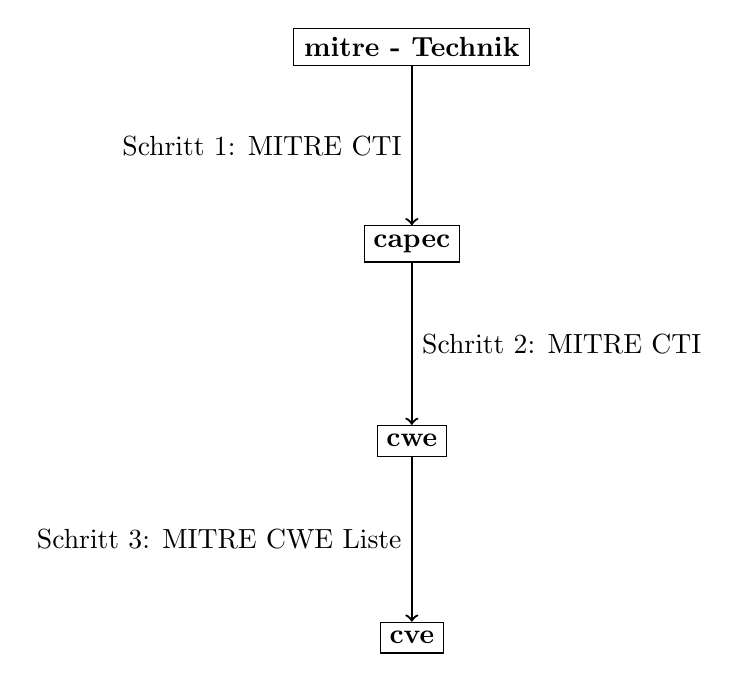
\begin{tikzpicture}[node distance=2cm, auto]
        % Nodes
        \node [rectangle, draw, text centered, minimum width=3cm] (mitre) {\textbf{\gls{mitre} - Technik}};
        \node [rectangle, draw, below of=mitre, yshift=-0.5cm] (capec) {\textbf{\gls{capec}}};
        \node [rectangle, draw, below of=capec, yshift=-0.5cm] (cwe) {\textbf{\gls{cwe}}};
        \node [rectangle, draw, below of=cwe, yshift=-0.5cm] (cve) {\textbf{\gls{cve}}};
        % Arrows
        \draw[->, thick] (mitre) -- (capec) node[midway, left] {Schritt 1: MITRE CTI};
        \draw[->, thick] (capec) -- (cwe) node[midway, right] {Schritt 2: MITRE CTI};
        \draw[->, thick] (cwe) -- (cve) node[midway, left] {Schritt 3: MITRE CWE Liste};
    \end{tikzpicture}
    \caption{Ablauf des Mappings von MITRE-Technik zu spezifischen CVE-Datum über die Kategorisierungssysteme MITRE, CAPEC, CWE und CVE.}
    \label{fig:mitre_mapping}
\end{figure}

Die spezifischen Angriffe, die im Dashboard angezeigt werden, stammen aus dem \gls{foran} Attack-Tool. Ein Überblick darüber wurde in Kapitel \ref{sec:tech-foran} gegeben. \todo{Ist das wirklich so??}

\par Das Attack-Tool implementiert aktuell circa 250 Szenarien die Angriffsspuren erzeugen. Diese werden in 38 Techniken sortiert und übergeordnet auf 10 Taktiken verteilt. Eine Technik kann dabei in mehreren Taktiken angewendet werden. Anhang \ref{app:attack-szenarien} beinhalten die Szenarien und, wenn vorhanden, die Zuweisungen zu einer \gls{mitre}-Technik. Nicht jeder dieser Angriffe lässt sich einer \gls{mitre}-Technik\footnote{Wenn ohne weitere Information von einer \gls{mitre}-Technik oder Taktik die Rede ist, meint das im Rahmen dieser Arbeit Inhalte des \gls{attack}-Frameworks.} zuordnen. Es existieren neben diesem noch andere Frameworks von \gls{mitre} selbst oder von Dritten abgewandelte Versionen, die auf einen spezifischen Anwendungsfall abzielen. In der \glqq{}\gls{tm4k}\grqq{} von Microsoft werden Kubernetes spezifische Angriffstechniken behandelt \autocite{TacticsThreatMatrix}. Teilweise tragen die Techniken einen anwendungsspezifischen Namen und referenzieren eine existierende \gls{mitre}-Technik, wie zum Beispiel bei \gls{mitre}-Technik \glqq{}T1070: Indicator Removal\grqq{} und \gls{tm4k}-Technik \glqq{}T1070: Delete Kubernetes events\grqq{} \autocite{IndicatorRemovalTechnique} \autocite{DeleteKubernetesEvents}. Einige sind jedoch so spezifisch, dass dazu bisher keine \gls{mitre}-Technik existiert und die neue Technik nur unter einer von Microsoft vergebenen ID (\textit{MS-TA-XXX}) verfügbar ist, wie im Fall von \glqq{}MS-TA9003: Kubeconfig file\grqq{} \autocite{KubeconfigFileThreat}. Zum jetzigen Zeitpunkt ist der in Abbildung \ref{fig:mitre_mapping} dargestellte \textit{Schritt 1} nur für Daten aus der \textit{Enterprise}-Matrix des \gls{attack}-Frameworks durch \gls{acema} implementiert. Auf eine Generalisierung für die Gesamtheit der \glspl{capec} wird in Kapitel \ref{sec:limitationen} eingegangen und eine eigene Implementierung in Kapitel \ref{sec:impl-anwendungVonAcema} vorgestellt.
\par Schritt 1 des in Abbildung \ref{fig:mitre_mapping} Ablaufs sucht für eine \gls{mitre}-Technik das zugehörige Angriffsmuster, den \gls{capec}.\todo{CAPEC sollte dann schon einmal im Technischen Hintergrund erkärt sein.} Die zugrundeliegenden Daten stammen aus dem von \gls{mitre} gepflegtem \gls{cti} Repository, in welchem die Daten regelmäßig aktualisiert im \textit{\gls{stix} 2.0}-Format veröffentlicht werden \autocite{IntroductionSTIX} \autocite{MitreCtiCyber}. Die durch \gls{acema} gefundenen \glspl{capec} zu den \gls{mitre}-Techniken sind jedoch nicht vollständig, eine Lösung dafür wird in Kapitel \ref{sec:impl-anwendungVonAcema} präsentiert. Schritt 2 nutzt dasselbe Repository, denn dort sind für das jeweilige \gls{capec}-Objekt auch zugehörige \glspl{cwe} unter externen Referenzen verknüpft \autocite{CtiUSAGEmdMaster}. In Schritt 3 wird über das Pythonmodul \textit{cwe2} nach zugehörigen \glspl{cve} gesucht. Die zugrundeliegenden Daten für diese Abfrage stammen aus der \gls{cwe} Liste, die regelmäßig von \gls{mitre} veröffentlicht wird. Diese Liste enthält auch zugehörige \glspl{cve}, die in diesem Kontext \glqq{}beobachtete Beispiele\grqq{} genannt werden \autocite{AboutcodeorgCwe22024} \autocite{CWEDownloads}.
\par Um weitere Informationen wie \gls{cvss}, Angriffsvektoren und Veröffentlichungsdatum über einzelne \glspl{cve} zu beschaffen, wird die \gls{nvd} des \gls{nist} über die Python Module \verb|cve_lookup| und \verb|nvdlib| abgefragt \autocite{NVDLibNVDLibNIST} \autocite{MachineThingCve_lookupLook} \autocite{NVDHome}. Die Ausgabe am Ende dieser Kette ist primär die \verb|json|-Datei, welche die Ergebnisse des Mappings enthält. Im Anhang \ref{app:acema-output} ist eine beispielhafte Ausgabe nach Ausführen von \verb|O-Cloud - Data Gathering.ipynb| gezeigt.
\par Wenn einem Artefakt vom Attack-Tool eine \gls{mitre}-Taktik zugewiesen ist, werden diesem Artefakt beim Start des Dashboards automatisch Information aus der \verb|json| Datei hinzugefügt. Diese weiteren Informationen sind nicht persistent, sondern werden jedes Mal neu evaluiert, wenn das Dashboard gestartet wird.
\todo{Hier noch weiter ausführen.}
\section{Auswahl der Visualisierungstechniken}
\todo{Auch hier Änderung des Kapitelnamens!}
\label{sec:auswahlDerVisualisierungstechniken}
Die Basis für die Wahl der Visualisierungstechniken im Dashboard wurden von Jonas Weber in seiner Arbeit gelegt \autocite{weberEvaluationDashboardTechniques}. \citeauthor{weberEvaluationDashboardTechniques} beschreibt darin grundlegende Prinzipien, die beim Design eines Dashboards eine wichtige Rolle spielen.
\par Das erste Prinzip beschreibt das Phänomen der präattentiven Wahrnehmung. Darunter versteht man die Wahrnehmung von visuellen Reizen, welches jedoch unterschwellig und ohne das Dazutun von Aufmerksamkeit passiert. Man spricht auch von Vorbewusstsein \autocite{PraeattentiveWahrnehmung}, \autocite{mallotWahrnehmungPraeattentiveIm2021}. Über das Design von Dashboard auf Basis dieses neurologischen Konzepts gibt es zahlreiche wissenschaftliche Arbeiten, hervorgehoben sei dabei die Übersicht von \citeauthor{barrera-leonHowPreattentiveProcess2023} \autocite{barrera-leonHowPreattentiveProcess2023}. Anwendung findet dieses Prinzip in der Implementierung des Dashboards zum Beispiel beim Design der Zeitleiste. Im Listing \ref{fig:cvss-colors} ist dargestellt, wie der Schweregrad von Metriken eines \glspl{cve} anhand einer farblichen Kategorisierung eingeordnet wird. Die Farbwahl beschränkt sich hierbei auf vier deutlich voneinander unterscheidbaren Farben \todo{Hier eventuell als Tabelle oder textit oder so...}: Grau für Keine Daten vorhanden, Grün für Niedriger Schweregrad, Gelb für Mittlerer Schweregrad, Rot für Hoher Schwerergrad. Wissenschaftlich ist die kategorische Wahrnehmung von Farben unter anderem durch die wissenschaftliche Arbeit von \citeauthor{cliffordColorCategoriesAffect2010} bewiesen \autocite{cliffordColorCategoriesAffect2010}. Die technische Implementierung der Farbkategorisierung ist in Kapitel \ref{sec:impl-cvssIntegration} erläutert.
%
\begin{figure}[H]
    \centering
    \includegraphics[width=0.8\textwidth]{cvss-colors}
    \caption{Farbkategorien zur Darstellung von Metriken}
    \label{fig:cvss-colors}
\end{figure}
%
\par Ein weiteres Prinzip, welches beim Visualisieren von Daten eine zentrale Bedeutung hat, wurde 1983 von \citeauthor{tufteBookReviewsVisual1984} als \textit{data-ink}-Prinzip definiert. Das Prinzip besagt, dass der Anteil der genutzten Farbe um die Daten darzustellen möglichst hoch sein soll. Damit soll die Darstellung von nicht-daten-bezogener \glqq Ausschmückung \grqq in der Visualisierung vermieden werden \autocite{tufteBookReviewsVisual1984}. An einem praktischen Beispiel kann jedoch gezeigt, dass ein geringeres \textit{data-ink} Verhältnis nötig sein kann, um Daten effizient darzustellen. In Kapitel \ref{sec:tech-foran} ist der Dateninhalt eines Artefaktes beschrieben. Als zentrale zu visualisierende Daten liegen jeweils das Start- und Enddatum der Artefakte vor. Die Abbildung \ref{fig:high-data-ink} zeigt die Darstellung von mehreren Artefakten auf einer Zeitleiste. Das \textit{data-ink} Verhältnis ist in dieser Darstellung sehr hoch, da tatsächlich nur die Start- und Endzeitpunkte dargestellt sind. Im Vergleich dazu wird in Abbildung \ref{fig:low-data-ink} die Zeitspanne zwischen den jeweiligen Daten eines Artefaktes zusätzlich farblich dargestellt. Es wird erkennbar, welche Punkte Start- oder Endpunkte sind. Dies war in Abbildung \ref{fig:high-data-ink} nicht intuitiv erkenntlich. Es ist in diesem Fall sinnvoll ein geringeres \textit{data-ink} Verhältnis zu erzielen, um Klarheit und Intuition zum Lesen zu schaffen. Die technische Konfiguration der Zeitleiste ist in Kapitel \todo{In welchem Kapitel kann ich darüber reden, aktuell passt keins...} erläutert.
%
\begin{figure}
    \centering
    \includegraphics[width=1\textwidth]{high-data-ink}
    \caption{Hohes \textit{data-ink} Verhältnis}
    \label{fig:high-data-ink}
\end{figure}
%
\begin{figure}
    \centering
    \includegraphics[width=1\textwidth]{low-data-ink}
    \caption{Niedriges \textit{data-ink} Verhältnis}
    \label{fig:low-data-ink}
\end{figure}
%
\par Diese beiden Prinzipien und \textit{best-practices} wurden auch bei Weiter- und Neuentwicklungen bei Visualisierung im Dashboard gewahrt. Bei der Darstellung des Angriffspfads und der Netzwerktopologie wurden bewusste design-technische Entscheidungen getroffen. Was genau unter diesen beiden neuen Visualisierungen zu verstehen ist, wurde in Kapitel \ref{sec:tech-foran} \todo{Oder leicht woanders, wenn es dort noch weitere Unterkapitel gibt.} bereits definiert. Die Angriffspfads-Visualisierung enthält nicht viele Daten, nimmt aber einen großen Platz auf der Detailübersicht eines Artefaktes ein. Der Angriffsgraph und Netzwerkgraph sind beim Laden der Seite nicht direkt, sondern nur nach einem bewussten Scrollen sichtbar. So wird der Nutzer nicht mit zu vielen Informationen auf einmal überladen. Die Graphen werden nicht als statische Bilder eingebettet. So lassen sich weitere Funktionen wie Tooltipps, dynamischer Zoom und die Verschiebbarkeit der einzelnen Elemente realisieren. Ein Tooltip hat hier die Funktion, zusätzliche hilfreiche Information zu liefern wenn der Nutzer mit dem Mauszeiger auf ein Element zeigt \autocite{TooltipCarbonDesign}. Die Darstellung eines Tooltips ist in Abbildung \ref{fig:tooltip} gezeigt. Über die Verschiebbarkeit der Elemente kann das Diagramm angepasst werden, um es verständlicher darzustellen oder für einen Export vorzubereiten. Die Graphen können über gängige Browser per \textit{Rechtsklick, Speichern unter / In neuem Tab öffnen} als \verb|.png| Datei exportiert werden.
%
\begin{figure}[H]
    \centering
    \includegraphics[width=0.5\textwidth]{tooltip}
    \caption{Tooltip auf einem Element im Angriffsgraphen}
    \label{fig:tooltip}
\end{figure}
%
\par Der Ablauf und das Ergebnis der Implementierung der Graphen sind in Kapitel \ref{sec:impl-visualisierungDesAngriffspfads} gezeigt.
\section{Entwicklungsumgebung}
\label{sec:Entwicklungsumgebung}
In diesem Kapitel wird etwas tiefer auf die Tools eingegangen, die zur Umsetzung der Implementierung des Dashboards genutzt wurden. Die generelle Architektur, genutzte Programmiersprachen und Technologien findet sich in Kapitel \ref{sec:tech-dashboard}. Zu Beginn wurde die Entwicklung auf einer rein lokalen Umgebung durchgeführt. Über das von MongoDB zur Verfügung gestellte \gls{cli} lief ein MongoDB-Server, ein per \verb|go build| gebaute Dashboard-Server und der per \verb|yarn dev| gestartete Vite-Entwicklungs-Server auf dem lokalen Rechner \autocite{MongoDBDeveloperData} \autocite{Vite}. Die Testdaten stammten aus dem Gitlab-Repo und sind von Jonas Weber zur Verfügung gestellt \autocite{AddExampleData2023}. Die Qualität und Menge der Testdaten waren für den Anfang ausreichend. Um auf aktuellen Daten zu arbeiten und näher an der etablierten Testumgebung zu sein, wurde ab dem 7. August 2024 eine \gls{vm} in der \glqq\gls{dnlab}\grqq-Umgebung der TH Köln genutzt. Das Arbeiten auf einem entfernten (\textit{en: remote}) Host innerhalb von \gls{vscode} wird seit 2019 durch eine von Microsoft entwickelte Erweiterung vereinfacht \autocite{RemoteSSHVisual}. Die Anwendung kann dann entweder weiterhin lokal auf der \gls{vm} oder zentralisiert per Ansible bereitgestellt (\textit{en: deployed} \todo[inline]{FIX ME}) werden \autocite{HomepageAnsibleCollaborative}. Ansible ist ein Tool zur Orchestrierung von Systemen und Software, welches durch die Ausführung von Skripten einen spezifischen technischen Zustand herstellt \autocite{ansiblecollaborativeetalHowAnsibleWorks2024}. Für die Ausführung des \gls{acema}-Quellcodes ist das Aufsetzen einer Python-Umgebung nötig \autocite{klement2023acema} \autocite{WelcomePythonorg}.

\section{Datenquellen}
\label{sec:datenquellen}
\todo{Eventuell dieses Kapitel eher unter technischen Hintergrund??}
\par Die \gls{tm4k}, bereitgestellt von Microsoft, ist eine spezialisierte Threat-Matrix für Kubernetes-Umgebungen, die verschiedene Angriffsvektoren und Schwachstellen in containerisierten Plattformen kategorisiert. Sie enthält detaillierte Informationen zu typischen Angriffstechniken, Taktiken und entsprechenden Verteidigungsmaßnahmen, die speziell für Kubernetes relevant sind \autocite{TacticsThreatMatrix}. Die Quelle wurde seit der Erstveröffentlichung 2020 bis Anfang 2023 regelmäßig aktualisiert, hat aber seitdem keine Updates mehr bekommen \autocite{DeploymentsMicrosoftThreatMatrixforKubernetes}. Die Quelle wird dennoch häufig genutzt und bietet eine hilfreiche Wissensquelle über die Angriffstechniken im Kubernetes Umfeld.

\todo{Nur relevant, wenn ich auch über die Testfälle (artifacts-testing) im Attacktool rede}
\par Die Redguard Matrix für Kubernetes bietet eine Übersicht über Sicherheitsrisiken und Angriffsvektoren, die in Kubernetes-Umgebungen auftreten können \autocite{KubernetesThreatMatrix}. Sie legt einen besonderen Fokus auf spezifische Angriffe und gibt für viele Techniken Kubernetes Manifeste und \gls{cli} Kommandos an, mit denen das eigene System auf die Schwachstelle getestet werden kann. Ihre Anwendung in der Schwachstellenanalyse von \oran kann hilfreich sein, da sie spezifische Ressourcen für das Finden von Schwachstellen im eigenen System enthält.

\par \gls{mitre}-\gls{attack} ist ein umfassendes Framework zur Klassifikation und Analyse von Cyberangriffen, das verschiedene Angriffstaktiken und -techniken systematisch erfasst. Sie stellt Informationen über Angriffsmethoden, betroffene Technologien und mögliche Gegenmaßnahmen bereit, die weltweit in der Sicherheitsforschung und -praxis genutzt werden. Die Quelle ist aufgrund ihrer breiten Akzeptanz und der kontinuierlichen Aktualisierung durch die \gls{mitre}-Organisation als äußerst verlässlich einzustufen. Für die Analyse von Schwachstellen in Open-RAN-Umgebungen ist sie, wie auch für andere Umgebungen, unverzichtbar, da sie eine universelle Struktur bietet, um Angriffe auf die Infrastruktur zu kategorisieren und gezielte Schutzmaßnahmen abzuleiten \autocite{MITREATTCK}.
%
\par In der Implementierung von \gls{acema} werden Daten aus externen Datenquellen genutzt. Für das Mapping von \gls{mitre}-Technik zu \gls{cve} wird das \gls{mitre}-\gls{cti} Repository genutzt. Weitere Informationen über einen spezifischen \gls{cve} werden über die \gls{nvd} des \gls{nist} beschafft.
\par Das \gls{cti} Repository enthält eine Vielzahl an Daten zur Identifikation und Kategorisierung von Cyberangriffstechniken. Es stellt spezifische Zuordnungen zwischen den im \gls{mitre} \gls{attack}-Framework beschriebenen Angriffstechniken und Schwachstellen (\glspl{cwe}) bereit, die eine wichtige Grundlage für Bedrohungsanalysen bilden. Diese Informationen umfassen unter anderem Angriffsmethoden, Exploit-Beschreibungen und potenzielle Abwehrmaßnahmen. Wissenschaftlich anerkannt ist das Repository durch die breite Akzeptanz des \gls{mitre} \gls{attack}-Frameworks in der Sicherheitsforschung sowie durch die Anwendung in praxisorientierten Sicherheitslösungen.
\par Die \gls{nvd} ist eine zentrale Datenbank des \gls{nist}, die umfassende Informationen zu Schwachstellen und deren Bewertungen liefert. Sie basiert auf international anerkannten Standards wie CVE und CVSS, um die Schwere und Ausnutzbarkeit von Sicherheitslücken zu quantifizieren. Die NVD ist aufgrund ihrer Verlässlichkeit \todo{Link zu Einschränkungen} und der Bereitstellung standardisierter Sicherheitsmetriken ein unverzichtbares Werkzeug in der Sicherheitsforschung und -praxis. Die Kombination aus systematischer Datenaufbereitung und fundierten Bewertungen macht die NVD besonders geeignet für die Implementierung von Sicherheitslösungen und ist zum Beispiel standardmäßig in einigen der meistgenutzten Software in Enterprise Umgebungen integriert \autocite{AssetsNVDIntegration} \autocite{InformationenNVDIntegrationen}.

\section{Limitation}
\label{sec:limitationen}
Die Analyse und Implementierung unterliegt spezifischen Einschränkungen, die sowohl durch methodische als auch durch technologische Faktoren bedingt sind. Dabei sind insbesondere die Generalisierbarkeit der Ergebnisse und die Abdeckung aller relevanten Daten kritisch zu betrachten. \todo{Über "Generalisierbarkeit der Ergebnisse und die Abdeckung aller relevanten Daten" noch schreiben oder hier streichen.} Weiterhin beeinflussen die Auswahl und die Qualität der genutzten Datenquellen sowie deren Aktualität die Aussagekraft der Analyse. \todo{Diesen Absatz nochmal betrachten.}
\subsection{Generelle Limitationen}
\label{limitation-generell}
\par Die \gls{nvd} gilt als zentrale Resource für Informationen über öffentlich bekannte Sicherheitslücken. Daher scheint es auch als verlässliche Quelle für die IT-Sicherheitsbranche und Forschungszwecke. Laut einer Veröffentlichung vom 13. Februar 2024 kommt das \gls{nist} nicht der Abarbeitung der eingereichten \glspl{cve} hinterher und arbeitet daran, die Verzögerung bei der Analyse zu beheben \autocite{NVDProgramAnnouncement}. Am 13. November 2024 kündigte das \gls{nist} an, alle neu eingereichten \gls{cve} direkt verarbeiten zu können. Die Abarbeitung der zurückgestellten Daten dauert weiterhin an. Die Daten aus der \gls{nvd} sind daher aktuell  nicht auf dem neusten Stand \autocite{NationalVulnerabilityDatabase2024}. Eine vom \textit{IT Security Infrastructures Lab} der \textit{Friedrich-Alexander Universität Erlangen-Nürnberg} veröffentliche Studie vom \citedate{wunderNVDUsersAttitudes2024} unterlegt diese Feststellung mit empirischen Daten. Demnach sind fast 40\% der Befragten jährlich, monatlich, wöchentlich oder täglich von der verzögerten Veröffentlichung von neuen \glspl{cve} betroffen \autocite{wunderNVDUsersAttitudes2024}. Die damit zusammenhängenden und weitere technische Schwierigkeiten beeinflussen auch die Abfrageverfügbarkeit und Abfragegeschwindigkeit von Daten aus der \gls{nvd}. Für \gls{acema} haben die Einschränkungen weitreichende Konsequenzen, von verlangsamter Abfragegeschwindigkeit des \gls{cvss} für \glspl{cve} bis hin zur vollständigen Abwesenheit von \gls{cvss} Daten, die eine integrale Rolle für die Datenanalyse spielen.
%
\subsection{Limitation von ACEMA}
\label{limitationen-acema}
Die Implementierung von \gls{acema} nutzt für die Bewertung das \gls{cvss} in Version \textit{v2.0} aus dem Jahr 2007 \autocite[Zeile 75 - 80]{Acema_oranOCloud_Data_GatheringpyMaster}. Seit dem 27. Juni 2024 unterstützt die \gls{nvd} das Bereitstellen von Daten in \textit{v4.0} des \gls{cvss} \autocite{NVDCVSSV40}. Nicht nur ist die in \gls{acema} genutzte Version durch zwei \textit{major}-Versionen überholt, seit dem 13. Juli 2022 werden in der Datenbank keine neuen Angriffsvektordaten, qualitative Schweregrad-Bewertungen oder Schweregrad-Werte in \gls{cvss} \textit{v2.0} erstellt \autocite{RetirementCVSSV2}. Der Fall von unvollständigen Daten ist in der Bearbeitung dieses Projekts nicht vorgekommen, da alle im Ergebnisse des Mappings aufgeführten \glspl{cve} im Jahr 2021 oder früher veröffentlicht wurden. Es ist jedoch theoretisch möglich, dass diese Einschränkung bei der weiteren Nutzung dieser Methode zu fehlenden Daten führen kann.
%
\par Das von \gls{acema}, mithilfe des \gls{cti} Repositories, erstellte Mapping von \gls{mitre}-Technik zu \gls{capec} (Schritt 1 in Abbildung \ref{fig:mitre_mapping}) findet nicht alle \gls{capec}. Die Dokumentation im Repository erklärt zu dem Finden von \glspl{capec}: \gls{capec} IDs können dort für die Techniken gefunden werden, wo das unter externen Referenzen das Attribut \textit{source\_name} den Wert \verb|capec| hat \autocite{CtiUSAGEmdMaster} \autocite{CtiUSAGECAPECmdMaster}. \citeauthor{klementSecuring6GTransition2024} nutzen in ihrer Implementierung die Daten aus dem \textit{enterprise-attack/attack-pattern} Teil des Repositories \autocite{klement2023acema}. Nach demselben Prinzip kann auch der \textit{capec/2.1/attack-pattern} Teil des Repositories durchsucht werden. Der Unterschied in den beiden Datensätzen liegt darin, was der Hauptzweck der Daten ist. Der \textit{enterprise-attack} Teil enthält die Datenstruktur \todo{anderes Wort für Datenstruktur} der \gls{mitre} \gls{attack} \textit{Enterprise}-Matrix, mit Daten wie der \gls{mitre}-Technik ID, Taktik und angreifbare Platform sowie manchmal Referenzen zu \gls{mitre}-Techniken. Der \gls{capec} Teil enthält die Datenstruktur \todo{anderes Wort für Datenstruktur} des \gls{capec}-Frameworks, mit Daten wie \gls{capec} ID, Konsequenzen und Voraussetzungen für die Ausnutzung sowie manchmal Referenzen zu \gls{mitre}-Techniken. Es zeigt sich in den Daten aus Tabelle \ref{tab:comparison_with_diff}, dass über den \textit{\gls{capec}} Teil eine vollständigere Abbildung von \gls{mitre}-Technik zu \gls{capec} ID möglich ist. Die beiden Implementierungen des Mappings wurden auf demselben Datensatz aus Anhang \ref{app:mapping-dataset} ausgeführt, der ein direkter Export der Daten aus der Dashboardmatrix ist.
%

\begin{table}[H]
    \centering
    \caption{Vergleich der Daten zwischen eigener Implementierung und ACEMA Implementierung inklusive prozentualer Differenzen}
        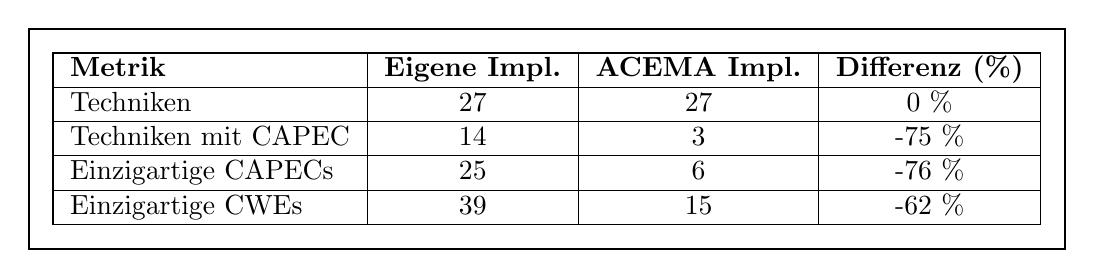
\begin{tikzpicture}
            \node[draw, thick, inner sep=3mm, rectangle] (table) {
            \begin{tabular}{|l|c|c|c|}
            \hline
            \textbf{Metrik} & \textbf{Eigene Impl.} & \textbf{ACEMA Impl.} & \textbf{Differenz (\%)} \\
            \hline
            Techniken & 27 & 27 & 0 \% \\
            \hline
            Techniken mit CAPEC & 14 & 3 & -75 \% \\
            \hline
            Einzigartige CAPECs & 25 & 6 & -76 \% \\
            \hline
            Einzigartige CWEs & 39 & 15 & -62 \% \\
            \hline
            \end{tabular}
        };
        \end{tikzpicture}
\label{tab:comparison_with_diff}
\end{table}